\chapter{Redes Neurais Artificiais}
\label{Cap:RedesNeurais}

Redes neurais talvez sejam umas das ferramentas mais importantes na aprendizagem de máquina. Sua capacidade de aproximar qualquer função, mesmo as não-contínuas~\cite{LIVRO:2009.9788591020805}, tornam-nas importantes ferramentas para classificação e predição de séries.

Existem redes de aprendizado supervisionado, onde a rede precisa da resposta certa no seu treinamento, e de aprendizado não-supervisionado, onde esse valor não é necessário. O~\emph{treinamento} de uma rede perceptron de múltiplas camadas permite o ajuste dos pesos da rede de forma que ela responda a estímulos similares com um erro minimizado. Como o perceptron de múltiplas camadas se baseia em um aprendizado supervisionado, é necessário dispor do valor esperado como resposta da rede dada uma entrada. 

\section{Perceptron de Múltiplas Camadas}

Em uma rede perceptron de múltiplas camadas, os neurônios estão contidos em conjuntos chamados~\emph{camadas}. Esquematicamente, as camadas são perfiladas paralelamente de forma que a primeira recebe o nome de~\emph{camada de entrada} e a última de~\emph{camada de saída}. Toda e qualquer camada que esteja entre a camada de entrada e a camada de saída é chamada de~\emph{camada intermediária} ou, mais comumente,~\emph{camada oculta}. A Figura~\ref{Fig:MlpEsquema} apresenta um exemplo de uma rede perceptron de múltiplas camadas.

\begin{figure}[htb]
  \centering
  \includegraphics[scale=0.75]{images/MlpEsquema.png}
  \caption{Um Perceptron de Múltiplas Camadas com três camadas. Dois neurônios na primeira, três na segunda e apenas um na terceira.}
    \label{Fig:MlpEsquema}
\end{figure}

Cada neurônio pertence unicamente a uma camada e se conecta a todos os neurônios da camada seguinte. Essas conexões possuem um valor atribuído, chamado de~\emph{peso}. Na Figura~\ref{Fig:MlpEsquema} cada neurônio é representado por um círculo amarelo, enquanto cada peso é representado por $P_{i,j}$.

O interior de um neurônio possui duas funções, a~\emph{função de agrupamento} e a~\emph{função de ativação}, também chamada de~\emph{função de transição} ou~\emph{função de propagação}. Excetuando-se os neurônios na camada de entrada, os demais recebem vários estímulos, como o resultado dos neurônios da camada anterior, bem como os pesos de conexão. A função de agregação de um neurônio soma o produto da saída dos neurônios da camada anterior com seus respectivos pesos de conexão, conforme Equação~\ref{Eq:FuncaoAgregacao}.

\begin{equation}
\displaystyle f_{ag} = \sum_{n=0}^{N} P_nS_n
\label{Eq:FuncaoAgregacao}
\end{equation}

Na Equação~\ref{Eq:FuncaoAgregacao}, $f_{ag}$ é a função de agregação de um neurônio qualquer, $N$ é o número de neurônios na camada anterior, $P_n$ é o peso de conexão entre o neurônio da camada anterior e o atual e $S_n$ é o valor calculado pelo neurônio da camada anterior. Imaginar $P$ como um vetor de pesos e $S$ como um vetor de valores calculados pelos neurônios da camada anterior permite reescrever a Equação~\ref{Eq:FuncaoAgregacao} conforme Equação~\ref{Eq:FuncaoAgregacaoVetor}, onde $P^T$ é o vetor transposto de $P$. 

\begin{equation}
\displaystyle f_{ag} = P^T . S
\label{Eq:FuncaoAgregacaoVetor}
\end{equation}

Já a função de transição recebe o resultado da função de agregação e o usa para calcular a saída do neurônio. A Figura~\ref{Fig:NeuronioEsquema} esquematiza o funcionamento interno de um neurônio. O neurônio da Figura~\ref{Fig:NeuronioEsquema} recebe a resposta de dois neurônios da camada anterior, bem como o peso de conexão entre cada um desses neurônios e o atual. 

\begin{figure}[htbp]
  \centering
  \includegraphics[scale=0.5]{images/NeuronioEsquema}
  \caption{Funcionamento interno de um neurônio, que recebe estímulo de dois neurônios da camada anterior.}
    \label{Fig:NeuronioEsquema}
\end{figure}

Diferente do que acontece com a função de agregação, existem diversas funções de ativação que podem ser usadas em um perceptron de múltiplas camadas \textcolor{red}{(ENCONTRAR UM TRABALHO QUE FAÇA UM ESTUDO COMPARATIVO ENTRE ESSAS FUNÇÕES, OU QUE USE MAIS DE UMA FUNÇÃO PARA CITAR AQUI)}. Inclusive, a última camada da rede pode ter uma função de transferência diferente das camadas anteriores, geralmente para normalizar a saída da rede~\cite{ARTIGO:2014.7078569}.

\section{O Algoritmo de Retropropagação}

O algoritmo de retropropagação\footnote{Também chamado por alguns autores de~\emph{propagação de retorno do erro}} foi proposto por~\textcolor{red}{ENCONTRAR ARTIGO DE QUEM PROPÔS E COLOCAR AQUI} e tem por objetivo modificar os pesos da rede de forma que a diferença entre o valor de saída da rede e o valor real, também chamado de~\emph{erro de predição}, seja o menor possível. Ele se baseia no uso de métodos de otimização, como o método do gradiente.

O treinamento de uma rede perceptron de múltiplas camadas precisa de dois vetores de valores, um de entrada e outro de saída. O algoritmo possui duas grandes etapas; a alimentação da rede e a retropropagação  do erro.

\subsubsection{Passo 1: Alimentação da rede}

O vetor de entrada é o estímulo a ser passado para a rede; ele tem o mesmo tamanho da camada de entrada. Dessa forma, cada valor do vetor é passado diretamente para um neurônio, sem utilizar a função de agregação. A Figura~\ref{Fig:skapura1996building} (retirada de~\cite{LIVRO:1996.skapura1996building}) ilustra como isso é feito esse processo.

A saída de um neurônio é o valor da função de ativação nele presente. Se o neurônio estiver presente na camada de entrada ou em uma camada oculta, esse valor é passado a todos os neurônios da camada seguinte, cujas funções de agregação calculação o valor a ser passado para a sua função de ativação. Se o neurônio estiver presente na camada de saída, o valor calculado pelo neurônio será a resposta da rede naquele neurônio.

\begin{figure}
\centering
\includegraphics[scale=1]{images/skapura1996building.png}
\caption{Ilustração retirada de~\cite{LIVRO:1996.skapura1996building} onde o valor de cada pixel é enviado para um neurônio na camada de entrada}
\label{Fig:skapura1996building}
\end{figure}

\subsubsection{Passo 2: Retropropagação do erro}

Uma vez terminado o passo 1, a última camada da rede possui suas respostas para o estímulo passado. Tais respostas precisam ser comparadas com o vetor de saída, que possui as respostas esperadas pela rede. Dessa forma, o vetor de saída precisa ser do mesmo tamanho da camada de saída da rede.

A função de erro mais comum a ser utilizada para comparar a resposta da rede com o vetor de saída~\textcolor{red}{ENCONTRAR ARTIGO QUE DIGA ISSO} é o erro quadrático (Equação~\ref{Eq:ErroQuadratico}, onde $i$ é índice de um neurônio na camada de saída, $y_i$ é o valor esperado para este neurônio e $S_i$ é o valor que a rede respondeu.

\begin{equation}
E = \frac{1}{2} \sum_i (y_i - S_i)^2
\label{Eq:ErroQuadratico}
\end{equation}

Deseja-se saber o quanto modificar o peso $P_{i, j}$ na camada de saída modifica o erro $E$ (Equação~\ref{Eq:ErroQuadratico}). Matematicamente, isso pode ser expressado pela Equação~\ref{Eq:DerivadaParcialDoErroEmRelacaoAoPeso}. A Equação~\ref{Eq:DerivadaParcialDoErroEmRelacaoAoPesoExpansao} possui a expansão através da aplicação da regra da cadeia.

\begin{gather}\label{Eq:DerivadaParcialDoErroEmRelacaoAoPeso}
\frac{\partial E}{\partial P_{i,j}} \\ \label{Eq:DerivadaParcialDoErroEmRelacaoAoPesoExpansao}
\frac{\partial E}{\partial P_{i,j}} = \frac{\partial E}{\partial S_{i,j}} * \frac{\partial S_{i, j}}{\partial E_{i,j}} * \frac{\partial E_{i,j}}{\partial P_{i,j}}
\end{gather}

O primeiro termo da Equação~\ref{Eq:DerivadaParcialDoErroEmRelacaoAoPeso}

\subsection{Um exemplo numérico}